\documentclass[11pt,a4paper]{article}
\usepackage[margin=2.6cm]{geometry}
\usepackage{amsmath,amssymb,bm,graphicx,booktabs}
\usepackage[colorlinks=true,linkcolor=blue,citecolor=blue]{hyperref}
\usepackage{enumitem}

\newcommand{\Pir}[1]{\Pi^{(\mathrm r)}_{#1}}
\newcommand{\Pis}[1]{\Pi^{(\mathrm s)}_{#1}}
\newcommand{\kt}{k_t}
\newcommand{\Qs}{Q^{*}}

\title{\vspace{-1.2em}Kernel energy allocation under mean strain:\\
results of the three discriminating tests}
\author{Sparsh Sharma (DLR Braunschweig)\\[0.2em]
\normalsize Results note --- follows the derivation note of 26 August --- \today}
\date{}

\begin{document}
\maketitle
\vspace{-2em}

\paragraph{Summary.} The three allocation routes --- the isotropic
$\alpha$-kernel (\texttt{ISO}), the strain-biased generalization of Fluids
\S6.2 (\texttt{CHI}), and Fistler et al.'s eddy types (\texttt{TYPES}) ---
were implemented as the single substitution $X_i^2=4S\Qs_i$ in the kernel
coefficients and run as $8\times1024$-realization ensembles under plane
strain on DLR CARO, with an unstrained ODT precursor and the strain rate
matched to the DNS values $Sk/\varepsilon\in\{16,\,0.8\}$. Outcome in one
sentence: \emph{every route reproduces exact rapid distortion in the rapid
limit, all routes return the Reynolds stresses toward isotropy by about
ten percent at $Sk/\varepsilon=0.8$, and none of them makes the transverse
spectral splitting $\phi_{11}/\phi_{33}$ depend on wavenumber --- the
splitting is rigid for every allocation rule, while the DNS splitting is
strongly scale-dependent.} The allocation is therefore not the lever for
the spectral distortion; where that leaves the model is discussed at the
end, with two questions for you.

\section{What was run}

\paragraph{Code.} In \texttt{set\_kernel\_coefficients} the available
energies $Q_i=P_i^2/4S$ are formed and the kernel amplitudes set from
$X_i=\sqrt{4S\Qs_i}$ with
\begin{align}
  \texttt{ISO}:&\quad \Qs_i=(1-\alpha)Q_i+\tfrac{\alpha}{2}(Q_j+Q_k),\ \ \alpha=\tfrac23
  \ (\chi=0), \\
  \texttt{CHI}:&\quad \Qs_i=\tfrac{Q}{3}+\chi\bigl(Q_i-\tfrac{Q}{3}\bigr)+\beta\hat A_{ii}Q,
  \ \ \chi=0,\ \beta=0.3, \\
  \texttt{TYPES}:&\quad \Qs_j=(1-\alpha_2)Q_j+\alpha_2Q_k,\ \Qs_k=(1-\alpha_2)Q_k+\alpha_2Q_j,\ \Qs_m=Q_m,
  \ \ \alpha_2=\tfrac12,
\end{align}
the omitted component $m$ sampled with $p_m=\tfrac13$ (\texttt{TYPESeq})
or $p=(\tfrac14,\tfrac14,\tfrac12)$ (\texttt{TYPESw}, which breaks the
$u\leftrightarrow w$ symmetry by omitting $w$ half the time). $\Qs_i$ is
clipped at zero and renormalized to $\sum_i\Qs_i=Q$; the eddy time scale
$\tau$ and the continuous rapid operator $\dot u=(-A+B)u$ are untouched.
\texttt{ISO} is bit-identical to the original code. The line is the $x_2$
(compression) axis of $A=S\,\mathrm{diag}(\tfrac12,-\tfrac12,0)$ and
dilates with it, $L(e)=L_0e^{-e/2}$.

\paragraph{A first campaign, and why it was inconclusive.} With the strain
switched on at $t=0$, every case --- both strain rates, all modes --- gave
the same $b_{22}(e)$ and a wavenumber-rigid splitting. The eddy logs
explained it: the band-limited spectral initial condition relaxes through a
burst of $\sim65$ accepted eddies in $t<0.05$ that loses three quarters of
$\kt$, after which the line is nearly eddy-free (at $S=0.5$ only $\sim7$
eddies per line over $e\in[0.25,1]$). Both the ``rapid'' and the ``slow''
runs were burst $+$ rapid operator; the slow term the allocation governs
was effectively absent, and the modes could not be told apart.

\paragraph{Precursor and rate matching.} A strain-onset time
\texttt{tStrainOn} was added (before it the run is plain ODT: zero strain
source, no dilatation, no strain bias in \texttt{CHI}). An unstrained
pilot (64 realizations) gave the relaxed state: the burst is over by
$t\approx0.2$; afterwards $\kt/\varepsilon\approx1.2\,t$ with
$\varepsilon=\nu\sum_i\langle(\partial u_i/\partial y)^2\rangle$, and the
eddy coverage time $1/(\text{rate}\times\text{size})$ agrees with
$\kt/\varepsilon$ to 10--30\%, so the ODT analogue of $Sk/\varepsilon$ is
unambiguous. Onset at $t=0.4$, where $\kt/\varepsilon=0.41$, then
\begin{center}
\begin{tabular}{lcccc}
\toprule
 & $S$ & $S\kt/\varepsilon$ & eddies per line in $e\le1$ & size \\
\midrule
rapid & 40 & 16  & 0.7 & --- \\
slow  & 2  & 0.8 & 6.7 (0.6 line coverages) & $0.09\,L$ \\
\bottomrule
\end{tabular}
\end{center}
The onset state at 1024 realizations is isotropic,
$b=(-0.005,+0.003,+0.002)\pm0.003$; all anisotropies below are
$b_{ij}(e)-b_{ij}(0)$. Dumps at $e=0,\tfrac14,\tfrac12,\tfrac34,1$;
jackknife errors over realizations.

\section{Results}

\begin{table}[h!]
\centering\small
\begin{tabular}{l|cc|cc}
\toprule
 & \multicolumn{2}{c|}{rapid, $S\kt/\varepsilon=16$} & \multicolumn{2}{c}{slow, $S\kt/\varepsilon=0.8$}\\
mode & $\mathrm db_{22}/\mathrm de|_0$ & $\Delta b_{22}(1)$ & $\mathrm db_{22}/\mathrm de|_0$ & $\Delta b_{22}(1)$\\
\midrule
\texttt{ISO}     & 0.133 & 0.123 & 0.130 & 0.110 \\
\texttt{CHI}     & 0.129 & 0.120 & 0.083 & 0.097 \\
\texttt{TYPESeq} & 0.133 & 0.124 & 0.135 & 0.109 \\
\texttt{TYPESw}  & 0.131 & 0.123 & 0.139 & 0.117 \\
\midrule
RDT exact (Cauchy) & 0.133 & 0.123 & 0.133 & 0.123 \\
DNS $128^3$        & $\approx0.15$ & 0.124 & --- & 0.125 \\
\bottomrule
\end{tabular}
\caption{Tests 1 and 2. Errors $\pm0.003$ (rapid) and $\pm0.004$ (slow) on
$\Delta b_{22}(1)$; $b_{33}$ stays within $\pm0.006$ of zero in every case.}
\label{tab:t12}
\end{table}

\begin{table}[h!]
\centering\small
\setlength{\tabcolsep}{4.5pt}
\begin{tabular}{lcccccccc|c}
\toprule
$\kappa_2(e)/\kappa_c(0)$ & 0.3--0.5 & 0.5--0.75 & 0.75--1.2 & 1.2--1.9 & 1.9--3 & 3--4.8 & 4.8--7.6 & 7.6--12 & integrated\\
\midrule
DNS $128^3$      & ---    & $-0.36$ & $-0.35$ & $-0.30$ & $-0.23$ & $-0.18$ & $-0.10$ & $+0.02$ & $-0.32$\\
\texttt{ISO}     & $-0.32$ & $-0.32$ & $-0.30$ & $-0.35$ & $-0.34$ & $-0.36$ & $-0.31$ & $-0.21$ & $-0.33$\\
\texttt{CHI}     & $-0.31$ & $-0.27$ & $-0.17$ & $-0.20$ & $-0.21$ & $-0.23$ & $-0.30$ & $-0.27$ & $-0.27$\\
\texttt{TYPESeq} & $-0.35$ & $-0.30$ & $-0.38$ & $-0.34$ & $-0.34$ & $-0.33$ & $-0.32$ & $-0.32$ & $-0.34$\\
\texttt{TYPESw}  & $-0.39$ & $-0.36$ & $-0.36$ & $-0.37$ & $-0.38$ & $-0.42$ & $-0.35$ & $-0.41$ & $-0.37$\\
\bottomrule
\end{tabular}
\caption{Test 3: transverse splitting $\phi_{11}/\phi_{33}-1$ at
$S\kt/\varepsilon=0.8$, $e=1$, in bands of $\kappa_2$ normalized by each
system's own $e=0$ energy centroid (both dilate by $e^{e/2}$). Band scatter
of the ODT values is about $\pm0.04$.}
\label{tab:t3}
\end{table}

\begin{figure}[h!]
\centering
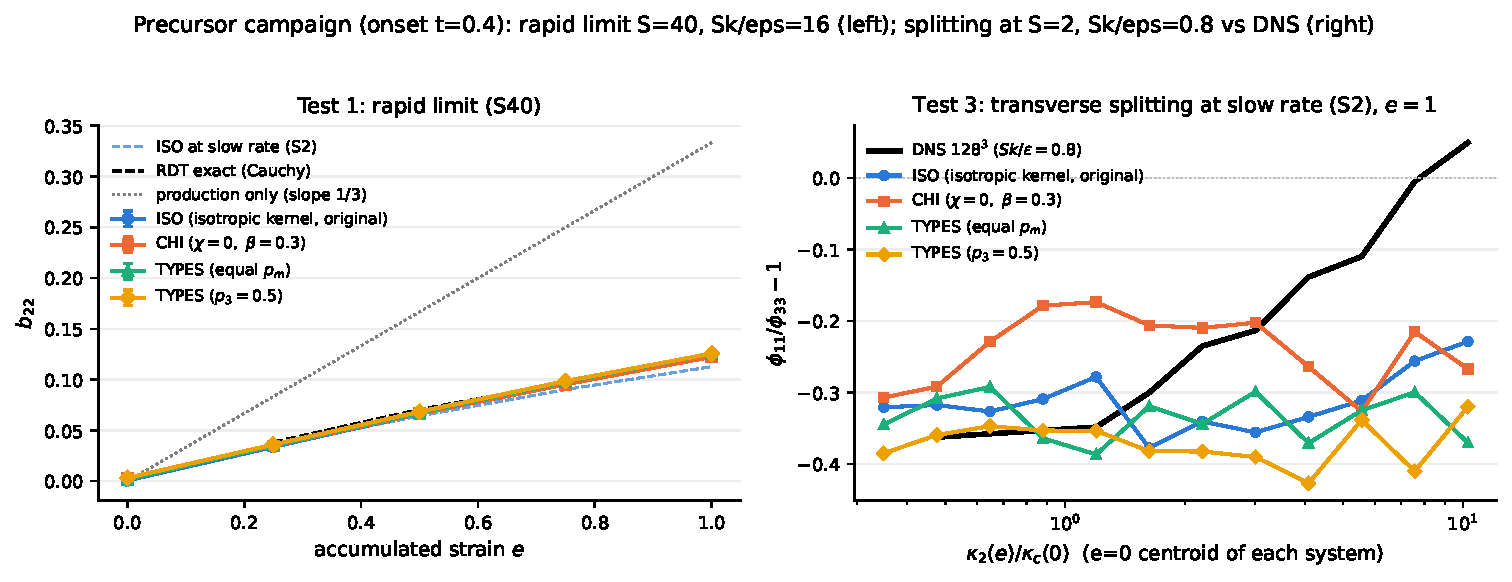
\includegraphics[width=\textwidth]{../post/closure_bound/odt_alloc/fig_alloc_tests_pre.pdf}
\caption{Left: Test 1, $b_{22}(e)$ per mode at $S\kt/\varepsilon=16$
against exact RDT (dashed) and production-only (dotted); the thin dashed
line is \texttt{ISO} at $S\kt/\varepsilon=0.8$. Right: Test 3, the
splitting of Table~\ref{tab:t3} against the DNS (black).}
\label{fig:tests}
\end{figure}

\section{Reading}

\paragraph{Test 1 --- the rapid term is untouched by every route.}
With under one eddy per line inside $e\le1$, all four modes sit on the
exact RDT curve to $\pm0.003$, \texttt{CHI} included. This is the
numerical confirmation of Conclusion~1 of the derivation note: the
allocation lives in the eddy event and cannot reach the rapid response;
the continuous operator carries it alone. (In the first campaign
\texttt{CHI} appeared to violate the rapid limit; that was its $\beta$
term acting on the burst eddies.)

\paragraph{Test 2 --- the slow term is there, and small.}
At $S\kt/\varepsilon=0.8$ the initial slopes of \texttt{ISO} and
\texttt{TYPES} are again the RDT value, and by $e=1$ the $\sim6.7$ relaxed
eddies have returned $b_{22}$ by about 10\% ($0.110$--$0.117$ against
$0.123$); the DNS at the same ratio shows no such deficit ($0.125$). The
routes differ from \texttt{ISO} by at most $0.013$: \texttt{TYPESw}
slightly above (omitting $w$ half the time leaves less exchange out of
$v$), \texttt{CHI} below. \texttt{CHI}'s reduced initial slope ($0.083$)
at the slow rate but not at the rapid rate is the signature of a per-eddy
term: $\beta\hat A_{ii}Q$ moves energy from the compressed component into
the stretched one at each eddy, at rate $\omega_e$, opposing the rapid
growth --- the ``form of the rapid term at the wrong rate'' the derivation
note warned about. As a slow-term bias it is legitimate but, at this
$\beta$, larger than the whole slow effect of the other routes.

\paragraph{Test 3 --- the splitting is rigid for every route.}
This is the decisive result and it is negative. The DNS splitting runs
from $-0.36$ at the energy-containing scales to zero and slightly positive
at ten times the centroid wavenumber: the small scales are isotropized by
the nonlinear transfer within one turnover. Every ODT route gives a flat
splitting across the same range, at the DNS \emph{integrated} value for
\texttt{ISO} and \texttt{TYPESeq} ($-0.33$, $-0.34$ against $-0.32$);
\texttt{TYPESw} is uniformly deeper, \texttt{CHI} uniformly shallower
(its $\beta$ term feeds $u$). ODT gets the total transverse anisotropy
right and its distribution over scales wrong, independently of how the
kernel energy is allocated.

\paragraph{Why.} Two structural facts, both now measured rather than
argued. The rapid operator is a wavenumber-independent linear map, so it
sets a splitting that is the same at every $\kappa_2$; the only
scale-local mechanism is the eddy, and the relaxed eddy population of
this line sits at one scale --- $0.09\,L$, which is the energy centroid
scale ($\kappa_c(0)=11.4$ waves per $L$) --- with no small-eddy population
at all (the pilot's eddy size grows monotonically as the line decays, and
the state at onset has $Re_\lambda\approx40$). Whatever the allocation
rule does, it acts at that one scale, and at the moment level it is a
10\% effect. A scale-selective return of the kind the DNS shows needs a
population of eddies smaller than the energy-containing scale, frequent
enough to act within one turnover; the allocation rule cannot supply the
population. I note that \texttt{TYPESw}, the route that breaks the
$u\leftrightarrow w$ symmetry by construction, changes the splitting's
level but not its shape either: symmetry breaking is not the missing
ingredient, scale selectivity is.

\section{Where this leaves the model, and two questions}

The two-term architecture is confirmed on both sides: the continuous
rapid operator is exact in the rapid limit and the eddy kernel is a
Rotta-type slow term. The manuscript's Reynolds-stress claims stand on
that. The spectral claim --- a broadband, scale-dependent distortion of
the upwash spectrum rather than a rigid one --- is not delivered by the
line model at this state, and \S6.2 allocation or eddy types do not change
that. Three ways forward, in the order I would try them:
\begin{enumerate}[leftmargin=2em,itemsep=2pt]
\item \emph{Broaden the eddy population before straining}: a forced or
  higher-$Re$ precursor whose relaxed state carries small eddies. If a
  scale-blind kernel then produces a $\kappa_2$-dependent splitting, the
  carrier of scale selectivity is the eddy-size distribution, which is a
  clean statement about the model; if not, the rigidity is structural.
\item \emph{Fistler et al.'s eddy time scale from the two participating
  components} (kept unchanged here). It changes the rate, not the scale
  structure, so I expect it to move Test~2 and not Test~3 --- but it is
  the one element of Route~D still untested.
\item \emph{Accept the division of labour}: ODT supplies the moment-level
  and integrated anisotropy, and the scale distribution comes from the DNS
  of Half~A (where the single-line closure is exact for axisymmetric
  strain and its plane-strain error is quantified). This is honest and
  defensible for the leading-edge application, whose response is
  dominated by the energy-containing scales where ODT is already right.
\end{enumerate}
The questions for you: (i) is there an ODT mechanism you would expect to
return the small scales selectively --- the size-dependence of the eddy
rate, the viscous cutoff, something in the kernel I have not considered
--- that I should test before concluding the rigidity is structural? (ii)
Do you see a reason to prefer a strain-orientation bias in the slow term
(Route~C) at all, given that at $\beta=0.3$ it already competes with the
rapid response at the slow rate?

\paragraph{Reproducibility.} Code (parameters \texttt{allocMode},
\texttt{allocChi}, \texttt{allocBeta}, \texttt{allocAlpha2},
\texttt{allocTypeProbs}, \texttt{tStrainOn}), the eight inputs
(\texttt{cases/odt\_pre/}), the analysis
(\texttt{post/closure\_bound/odt\_alloc/}) and the eddy statistics are in
the repository; ensembles are 116~MB per case and available on request.

\end{document}
